 %__       __ ________ ________ __    __  ______  _______   ______  __        ______   ______  __      __ 
%|  \     /  \        \        \  \  |  \/      \|       \ /      \|  \      /      \ /      \|  \    /  \
%| ▓▓\   /  ▓▓ ▓▓▓▓▓▓▓▓\▓▓▓▓▓▓▓▓ ▓▓  | ▓▓  ▓▓▓▓▓▓\ ▓▓▓▓▓▓▓\  ▓▓▓▓▓▓\ ▓▓     |  ▓▓▓▓▓▓\  ▓▓▓▓▓▓\\▓▓\  /  ▓▓
%| ▓▓▓\ /  ▓▓▓ ▓▓__      | ▓▓  | ▓▓__| ▓▓ ▓▓  | ▓▓ ▓▓  | ▓▓ ▓▓  | ▓▓ ▓▓     | ▓▓  | ▓▓ ▓▓ __\▓▓ \▓▓\/  ▓▓ 
%| ▓▓▓▓\  ▓▓▓▓ ▓▓  \     | ▓▓  | ▓▓    ▓▓ ▓▓  | ▓▓ ▓▓  | ▓▓ ▓▓  | ▓▓ ▓▓     | ▓▓  | ▓▓ ▓▓|    \  \▓▓  ▓▓  
%| ▓▓\▓▓ ▓▓ ▓▓ ▓▓▓▓▓     | ▓▓  | ▓▓▓▓▓▓▓▓ ▓▓  | ▓▓ ▓▓  | ▓▓ ▓▓  | ▓▓ ▓▓     | ▓▓  | ▓▓ ▓▓ \▓▓▓▓   \▓▓▓▓   
%| ▓▓ \▓▓▓| ▓▓ ▓▓_____   | ▓▓  | ▓▓  | ▓▓ ▓▓__/ ▓▓ ▓▓__/ ▓▓ ▓▓__/ ▓▓ ▓▓_____| ▓▓__/ ▓▓ ▓▓__| ▓▓   | ▓▓    
%| ▓▓  \▓ | ▓▓ ▓▓     \  | ▓▓  | ▓▓  | ▓▓\▓▓    ▓▓ ▓▓    ▓▓\▓▓    ▓▓ ▓▓     \\▓▓    ▓▓\▓▓    ▓▓   | ▓▓    
 %\▓▓      \▓▓\▓▓▓▓▓▓▓▓   \▓▓   \▓▓   \▓▓ \▓▓▓▓▓▓ \▓▓▓▓▓▓▓  \▓▓▓▓▓▓ \▓▓▓▓▓▓▓▓ \▓▓▓▓▓▓  \▓▓▓▓▓▓     \▓▓    
%.:..:..:..:..:..:..:..:..:..:..:..:..:..:..:..:..:..:..:..:.
\chapter{Methodology}
The project with be executed in the following sequence:
\begin{enumerate}[label=\roman*.]
	\item Simulate standard \gls{OFDM} on MATLAB over an \gls{AWGN} channel.
	\item Obtain average \gls{PAPR} performance of the simulated system.
	\item Simulate the \gls{OFDM} system over a Rayleigh fading channel.
	\item Simulate the \gls{OFDM} system over a Rician fading channel.
	\item Obtain \gls{BER} performance of all simulated systems.
	\item Use MATLAB's regression tools to derive an expression for the \gls{BER} curves generated.
\end{enumerate}

%,;,;,;,;,;,;,;,;,;,;,;,;,;,;,;,;,;,;,;,;
\section{OFDM Simulation}
The communication system will be modeled in MATLAB's Simulink for ease of visualization and implementation. The blocks in the diagrams that follow have analogs in \gls{simulink}'s Communication toolbox library.
\subsection{OFDM Transmitter}
The transmitter:
\begin{figure}[htpb!]
	\centerline{\resizebox{15cm}{!}{\input{Graphics/Methodology/OFDM_T_BLK.pdf_tex}}}
	\caption{OFDM Transmitter Block Diagram Implementation}
	\label{fig:ofdm_t_meth}
\end{figure}
\begin{figure}[htpb!]
	\centerline{\resizebox{!}{0.935\textheight}{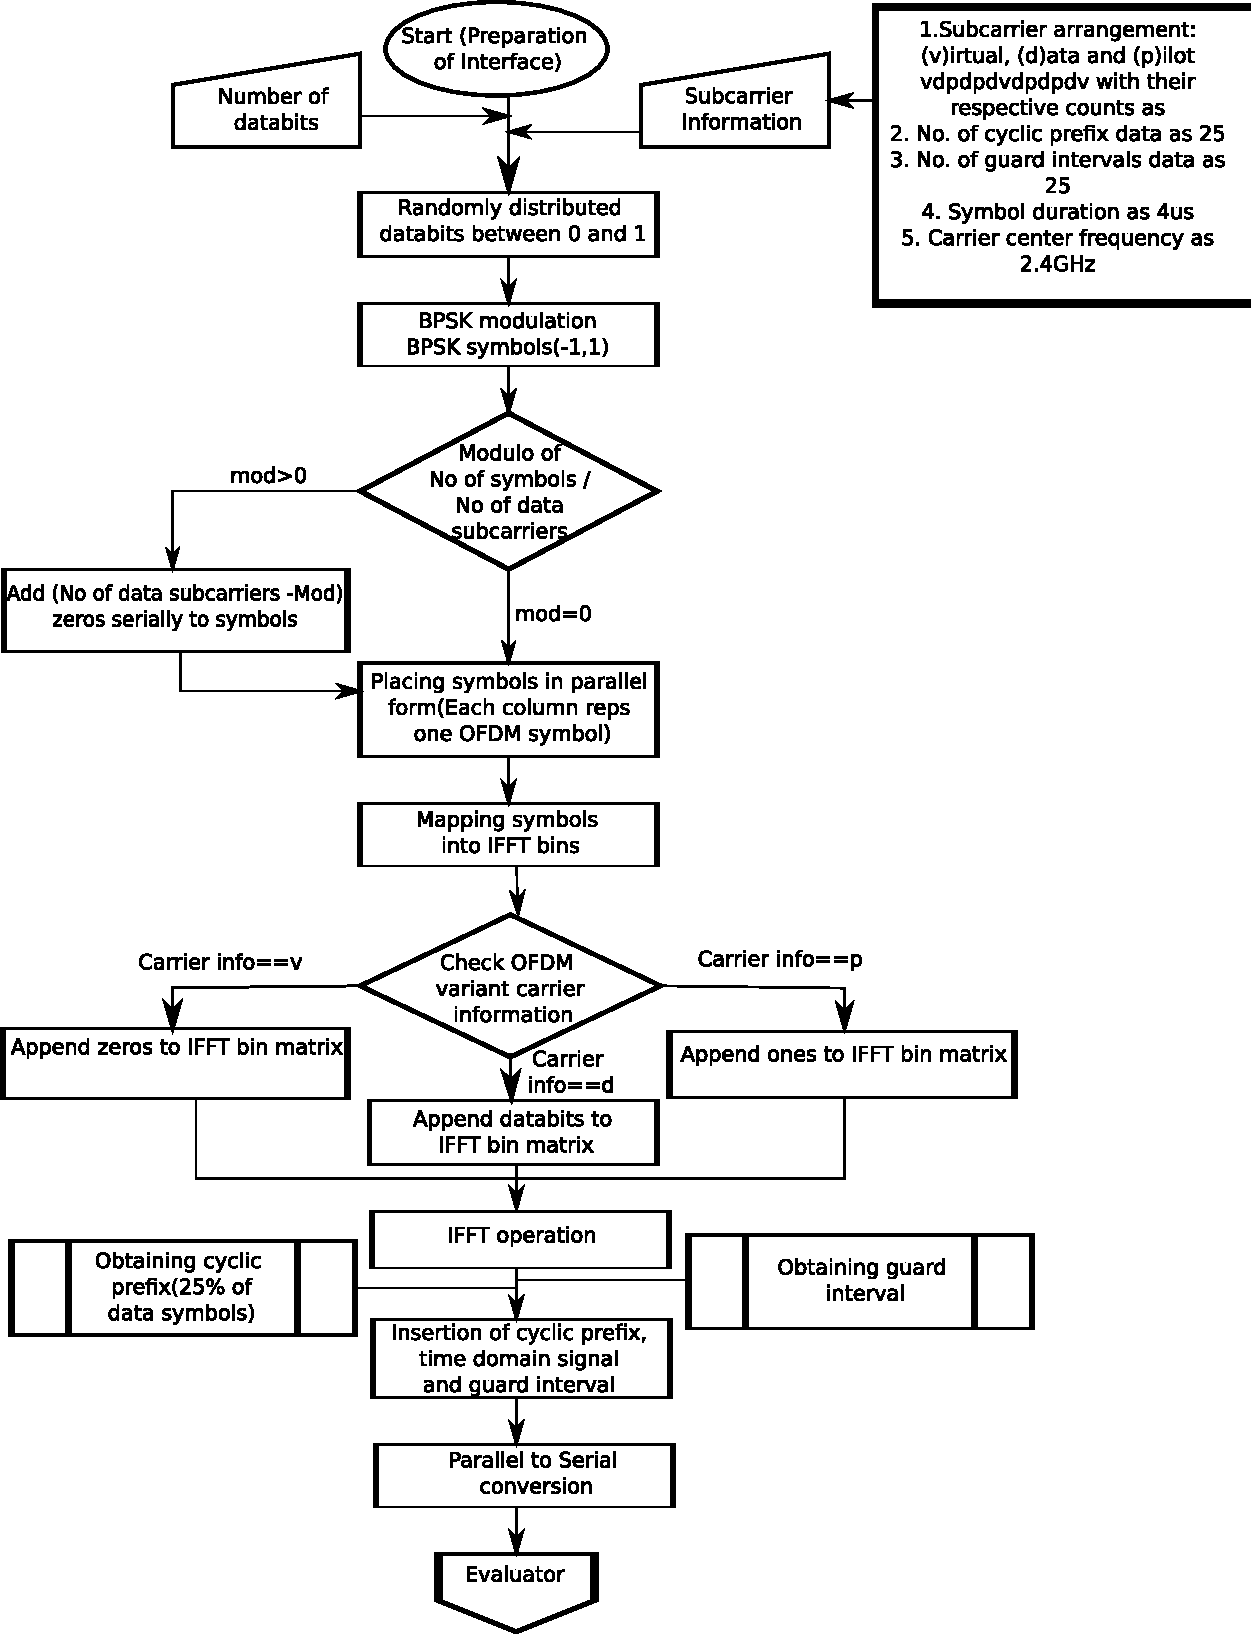
\includegraphics{Graphics/Methodology/Transmitter_flowchart.pdf}}}
	\caption{System Transmitter Flowchart Algorithm}
	\label{fig:system_transmitter}
\end{figure}

\pagebreak


\subsection{Channel}
The channel models that will be simulated are:
\subsubsection{AWGN Channel}
This channel adds white Gaussian noise to the signal as it is propagated through. 
\begin{figure}[htpb!]
	\centerline{\resizebox{15cm}{!}{\input{Graphics/Methodology/OFDM_CH_AWGN_BLK.pdf_tex}}}
	\caption{AWGN channel Block Diagram}
	\label{fig:ofdm_ch_awgn_meth}
\end{figure}

\subsubsection{Rayleigh Fading Channel}
The Rayleigh fading channel assumes no specular components in the transmitted signal. The signal Rayleigh fading has a Rayleigh Distribution.
\begin{figure}[htpb!]
	\centerline{\resizebox{15cm}{!}{\input{Graphics/Methodology/OFDM_CH_RAYL_BLK.pdf_tex}}}
	\caption{Rayleigh Fading Channel Block Diagram}
	\label{fig:ofdm_ch_rayl_meth}
\end{figure}

\subsubsection{Rician Fading Channel}
The Rician fading channel has multipath components as with the Rayleigh fading channel but has, in addition, a dominant line-of-sight component. The strength of the specular component determines the shape of the Rician distribution. 
\begin{figure}[h!]
	\centerline{\resizebox{15cm}{!}{\input{Graphics/Methodology/OFDM_CH_RICE_BLK.pdf_tex}}}
	\caption{Rician Fading Channel Block Diagram}
	\label{fig:ofdm_ch_rice_meth}
\end{figure}


\begin{figure}[htpb!]
	\centerline{\resizebox{!}{0.935\textheight}{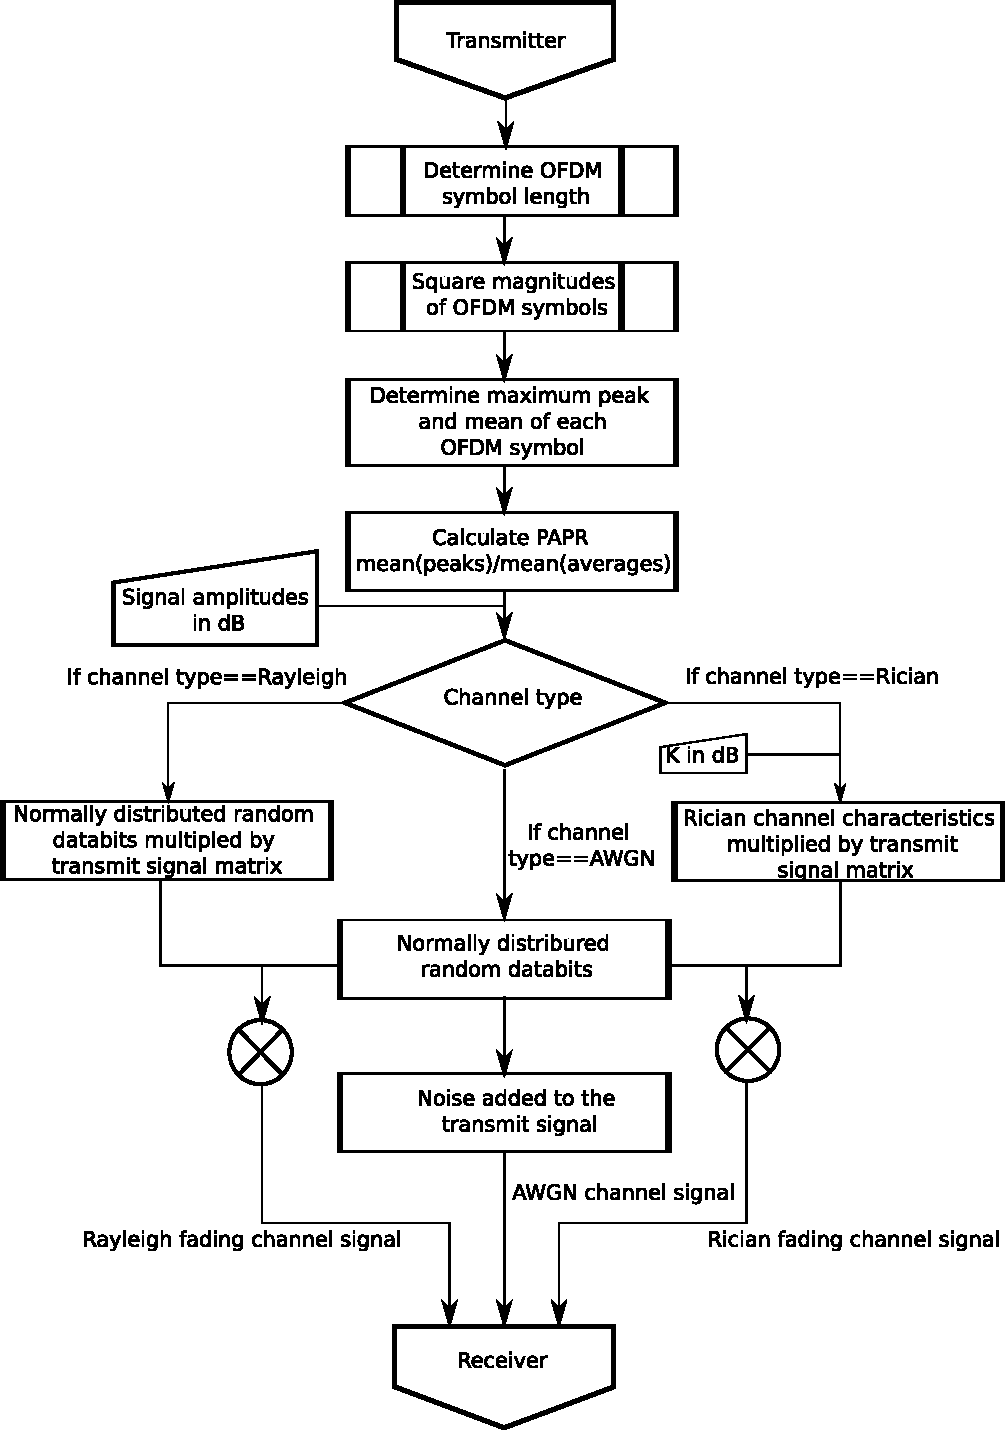
\includegraphics{Graphics/Methodology/Channel_flowchart.pdf}}}
	\caption{System Channel Flowchart Algorithm}
	\label{fig:ofdm_channel_meth}
\end{figure}
\pagebreak


\subsection{OFDM Receiver}
The receiver:
\begin{figure}[htpb!]
	\centerline{\resizebox{15cm}{!}{\input{Graphics/Methodology/OFDM_R_BLK.pdf_tex}}}
	\caption{OFDM Receiver Block Diagram Implementation}
	\label{fig:ofdm_r_meth}
\end{figure}
\begin{figure}[htpb!]
	\centerline{\resizebox{!}{0.935\textheight}{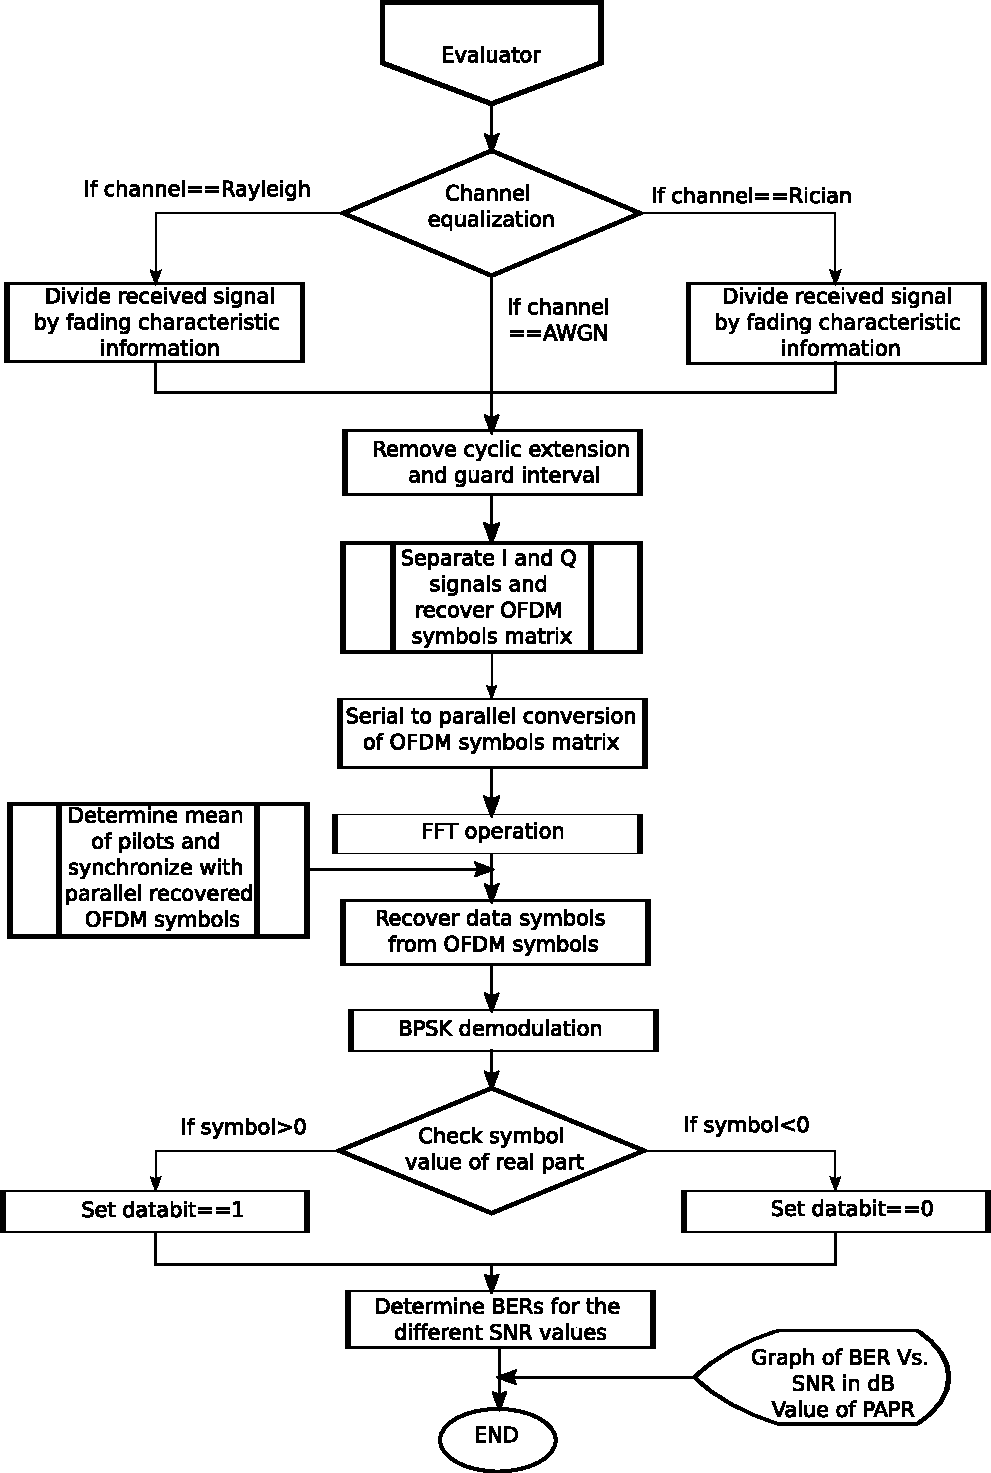
\includegraphics{Graphics/Methodology/Receiver_flowchart.pdf}}}
	\caption{System Receiver Flowchart Algorithm}
	\label{fig:ofdm_receiver_meth}
\end{figure}


\pagebreak

%,;,;,;,;,;,;,;,;,;,;,;,;,;,;,;,;,;,;,;,;
\subsection{BER Evaluation}
The system's \gls{BER} performance is to be evaluated within \gls{simulink} as well. The equivalent implementation would be as in figure \ref{fig:ber_blk_meth}
\begin{figure}[htpb!]
	\centerline{\resizebox{15cm}{!}{\input{Graphics/Methodology/BER_BLK.pdf_tex}}}
	\caption{\gls{BER} Evaluation}
	\label{fig:ber_blk_meth}
\end{figure}

%,;,;,;,;,;,;,;,;,;,;,;,;,;,;,;,;,;,;,;,;
\section{PAPR Evaluation}
\gls{PAPR} is evaluated at the transmitter output. To achieve this measurement, the peak amplitude is sampled over several symbol durations then its square divided by the square of the average signal amplitude.
\begin{figure}[!h]
	\centerline{\resizebox{10cm}{!}{\input{Graphics/Methodology/PAPR_BLK.pdf_tex}}}
	\caption{\gls{PAPR} Evaluation}
	\label{fig:papr_blk_meth}
\end{figure}
\pagebreak
%,;,;,;,;,;,;,;,;,;,;,;,;,;,;,;,;,;,;,;,;
\section{Curve fitting}

To determine the expressions for  the resulting BER curves from the system's simulation, \(Q\) function curves are fitted onto a line of best fit from the resulting BER data points:
\subsection{Gaussian Channel Model}

\begin{figure}[htpb!]
	\centering
	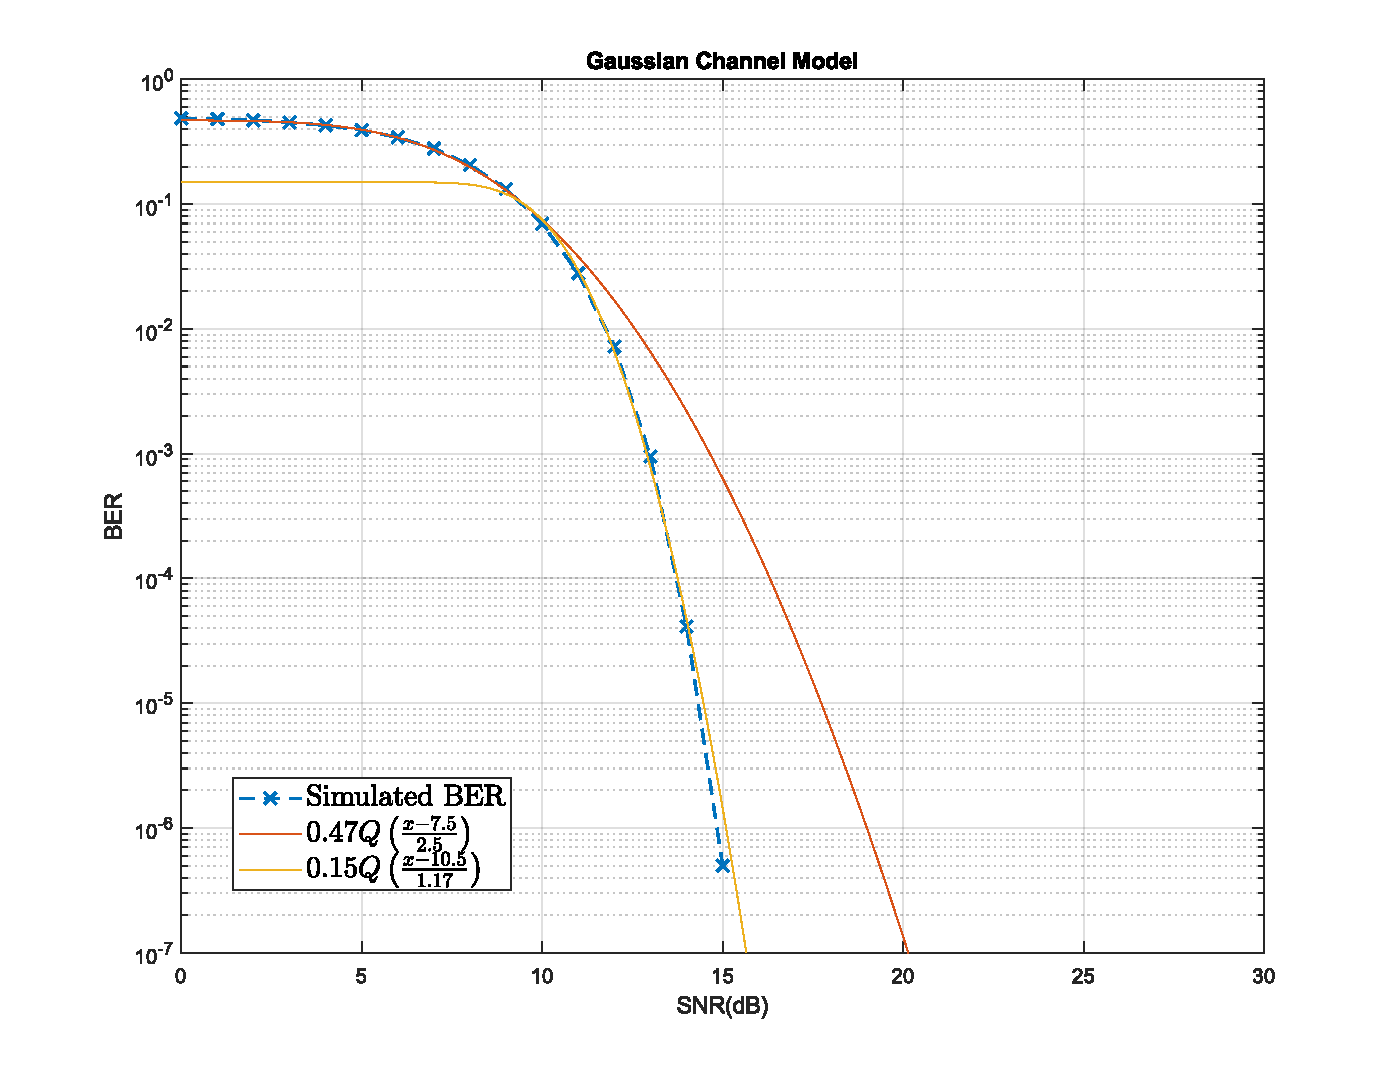
\includegraphics[scale=0.7]{Graphics/Methodology/GaussCurveFit.pdf}
	\caption{AWGN Channel curve fitting}
	\label{fig:gaussCurveFit}
\end{figure}
\pagebreak

\subsection{Rayleigh Channel Model}
\begin{figure}[htpb!]
	\centering
	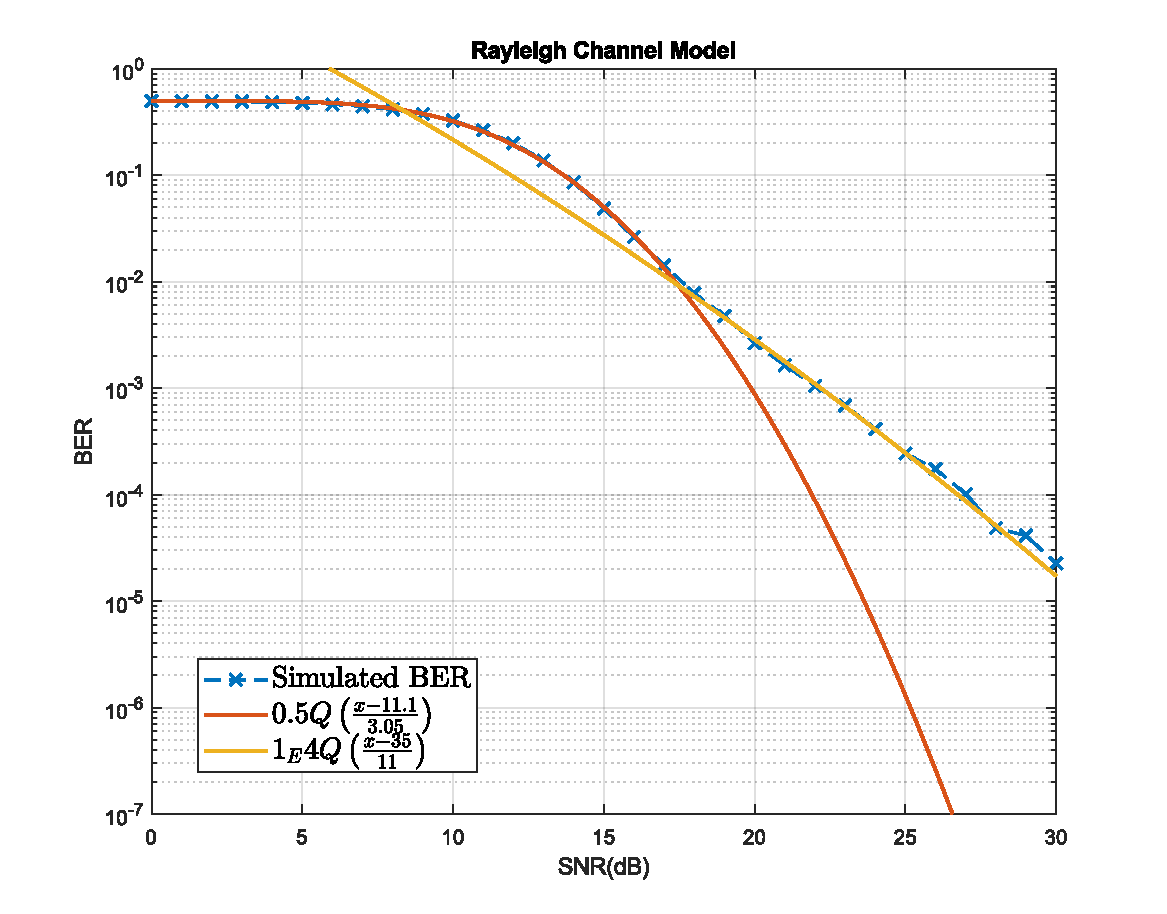
\includegraphics[scale=0.7]{Graphics/Methodology/RaylCurveFit.pdf}
	\caption{Rayleigh Channel Curve Fitting}
	\label{fig:gaussCurveFit}
\end{figure}

\subsection{Rician Channel Model}
\begin{figure}[htpb!]
	\centering
	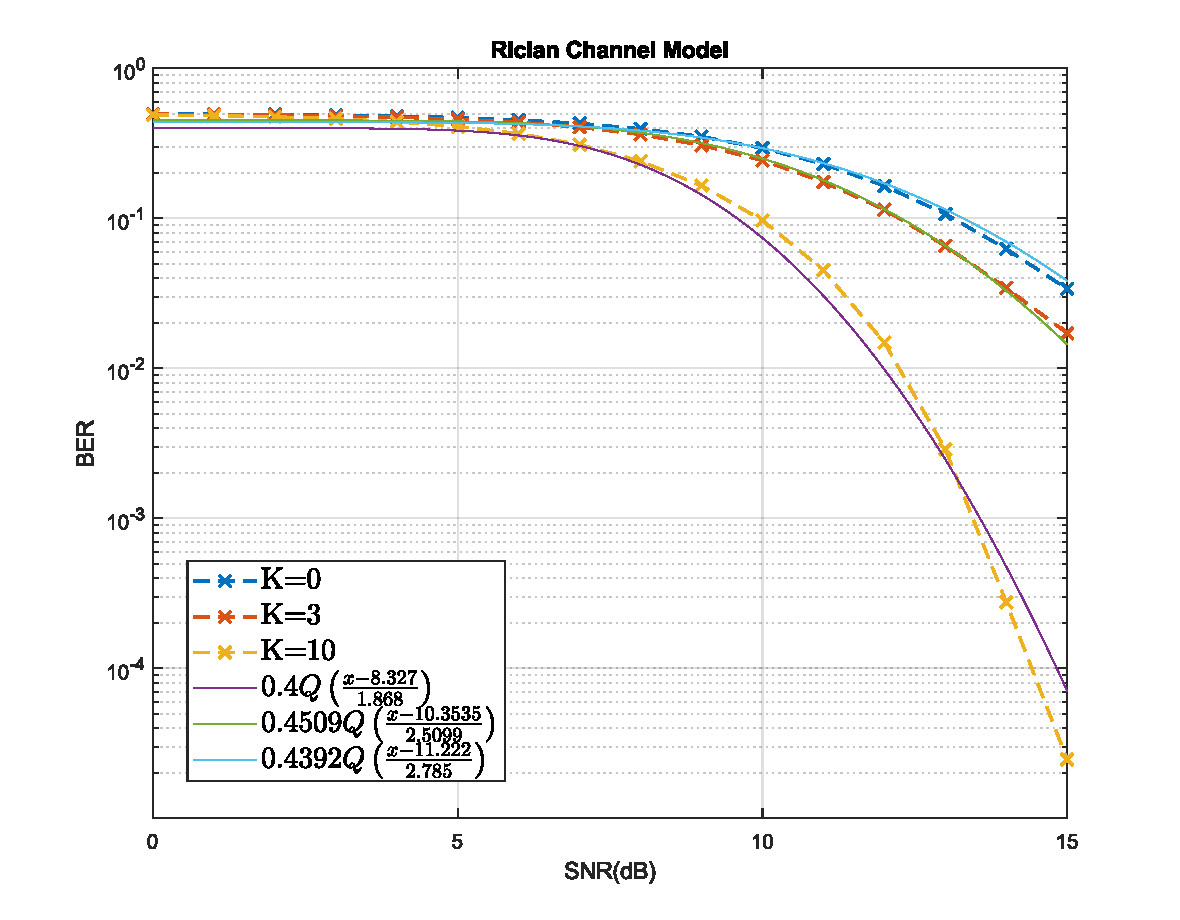
\includegraphics[scale=0.7]{Graphics/Methodology/RiceCurveFit.pdf}
	\caption{Rayleigh Channel Curve Fitting}
	\label{fig:gaussCurveFit}
\end{figure}
